\chapter{Method}
\label{ch:method}

This chapter describes our approach in four parts, mirroring the pipeline from raw data to trained model. First, the dataset is constructed by matching symbolic scores from three heterogeneous sources against an external graded repertoire database (Section~\ref{sec:dataset}). Second, a rhythm-alignment procedure recovers note durations for the PDF-derived scores, which carry pitch but no timing (Section~\ref{sec:rhythm_alignment}). Third, three successive generations of guitar-specific descriptors are engineered and audited (Section~\ref{sec:descriptors}). Finally, the additive RubricNet architecture is adapted to these descriptors and trained under an ordinal objective (Section~\ref{sec:model}).

\section{Dataset Construction}
\label{sec:dataset}
No existing resource pairs high-quality symbolic classical guitar scores with professional difficulty grades at a scale suitable for supervised learning. The dataset for this thesis was therefore assembled by matching symbolic scores from three separate corpora against an external graded repertoire database.

\subsection{Difficulty Labels}
Difficulty labels are taken from GuitarBurst~\cite{guitarburst}, an online database of graded classical guitar repertoire in which each work is assigned an integer difficulty from 1 (beginner) to 20 (advanced concert repertoire). Scraping the database produced 2{,}335 graded works, which serve as the label pool for matching. As a check on label quality, a sample of pieces at each difficulty level was manually reviewed by the author, an experienced guitarist; the assigned grades were plausible across the range, with disagreements limited to adjacent levels.

\subsection{Symbolic Score Sources}
Scores were collected from three sources with markedly different characteristics:
\begin{enumerate}
    \item \textbf{ClassClef PDFs}: vector-graphic tablature scores obtained from ClassClef, an online classical guitar score library. This is by far the largest source, but also the most problematic: parsing the PDFs recovers pitch, string, and fret reliably, while note durations are lost (Section~\ref{sec:rhythm_alignment}).
    \item \textbf{DadaGP}~\cite{sarmento2021dadagp}: a large corpus of GuitarPro tablature transcriptions in a tokenized format, of which only the classical guitar solo subset is relevant here.
    \item \textbf{GAPS}~\cite{riley2024gaps}: a small, high-quality corpus of classical guitar MusicXML scores aligned with audio recordings.
\end{enumerate}

\subsection{Matching and Deduplication}
Symbolic files were matched to GuitarBurst entries by fuzzy string matching on title and composer, with per-source matching procedures and a manual vetting pass over low-confidence matches. Since the same piece can appear in more than one source, cross-source duplicates were detected and removed (seven confirmed duplicates), along with one PDF whose musical content did not match its metadata. The final dataset contains \textbf{716 unique classical guitar pieces} spanning the full 1--20 difficulty range; Table~\ref{tab:dataset_sources} shows the source breakdown.

\begin{table}[htbp]
\centering
\caption{Dataset source distribution.}
\label{tab:dataset_sources}
\begin{tabular}{lr}
\toprule
\textbf{Source} & \textbf{Pieces} \\
\midrule
ClassClef PDFs & 655 \\
DadaGP (GuitarPro) & 49 \\
GAPS (MusicXML) & 12 \\
\midrule
\textbf{Total} & \textbf{716} \\
\bottomrule
\end{tabular}
\end{table}

\subsection{Difficulty Binning}
\label{sec:binning}
The raw 1--20 labels are heavily imbalanced: the middle of the scale is well populated (85 pieces at level 8), whereas the rarest levels contain very few pieces (levels 17--20 have 7, 8, 5, and 3 pieces, respectively); Figure~\ref{fig:label_distribution} shows the full distribution. Training directly on 20 classes was attempted and failed for precisely this reason (Section~\ref{sec:raw20}). The labels are therefore grouped into 8 ordinal classes by equal-frequency binning over contiguous level ranges:
\begin{equation*}
    \mathcal{C} = \{ [1\text{--}3],\ [4\text{--}5],\ [6\text{--}7],\ [8],\ [9\text{--}10],\ [11\text{--}12],\ [13\text{--}15],\ [16\text{--}20] \}
\end{equation*}
yielding class sizes between 37 and 136. The bin edges were fixed once, before any model development, and never changed thereafter.

\begin{figure}[htbp]
    \centering
    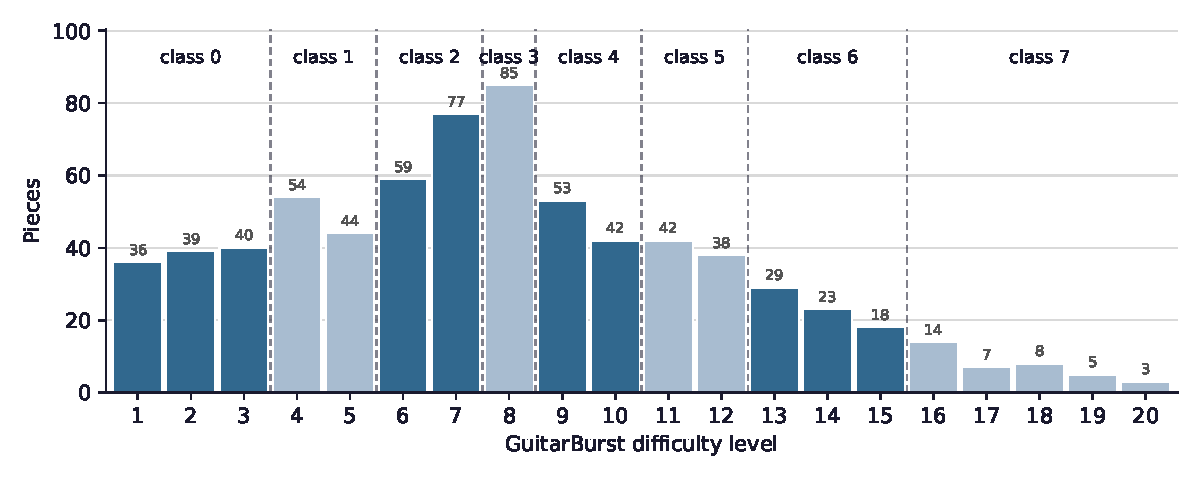
\includegraphics[width=\textwidth]{figures/label_distribution.pdf}
    \caption{Distribution of the raw GuitarBurst difficulty levels over the 716-piece dataset. Dashed lines mark the boundaries of the 8 ordinal classes produced by equal-frequency binning; alternating shades indicate bin membership. The sparsity of the highest levels (levels 17--20 hold 7, 8, 5, and 3 pieces) is what makes direct 20-level classification untenable (Section~\ref{sec:raw20}).}
    \label{fig:label_distribution}
\end{figure}

\subsection{Cross-Validation Splits}
All experiments use a single stratified 5-fold split over the binned labels, generated once and stored alongside the dataset. Every model in this thesis --- every baseline, every descriptor generation, every auxiliary experiment --- is trained and evaluated on these identical folds. Freezing the splits early was a deliberate safeguard against inadvertently tuning on test data over the many experimental iterations the project went through.

\section{Rhythm Alignment}
\label{sec:rhythm_alignment}
The PDF-derived scores, 655 of the 716 pieces, carry correct pitch, string, and fret information but no usable rhythm: the vector-graphics parsing cannot recover note durations, so every note initially emerges as a uniform quarter note, and the time signature defaults to 4/4. Any descriptor involving timing --- how fast a passage is, how much time a position shift has available --- cannot be computed on such data.

ClassClef also provides a separate collection of roughly 6{,}000 MIDI performances, not paired to the PDFs in any fixed way. To recover rhythm, each PDF is first matched to a candidate MIDI from this collection, and an alignment procedure then transplants the MIDI timing onto the PDF pitch sequence in four steps:
\begin{enumerate}
    \item \textbf{Pitch-sequence alignment.} The PDF's note sequence and the MIDI's note sequence are aligned with the Needleman--Wunsch algorithm (Section~\ref{sec:prelim_alignment}), whose tolerance for local insertions and deletions absorbs repeats, ornaments, and transcription discrepancies between the two renditions. Pieces whose best alignment covers too little of the score are rejected rather than force-matched.
    \item \textbf{Time signature.} The time signature is taken from the MIDI meta-events rather than from the PDF parser, whose 4/4 default is frequently wrong.
    \item \textbf{Duration from inter-onset intervals.} A note's duration is set to the inter-onset interval to the next note (Equation~\ref{eq:ioi}) rather than to its sounding duration in the MIDI. As discussed in Section~\ref{sec:prelim_representations}, guitar bass strings ring far past their notated values, so sounding durations systematically overstate how long notes are held; onsets are the reliable signal.
    \item \textbf{Serialization.} The aligned pitches with corrected timing are written back out as MusicXML.
\end{enumerate}

Figure~\ref{fig:alignment} illustrates the procedure on a short excerpt. The procedure aligned 579 of the 655 PDF pieces; the remaining 76 could not be used --- nearly all rejected for low alignment coverage, three because no matching MIDI file existed. Together with the sources that natively carry rhythm (all 12 GAPS scores and 48 of the 49 DadaGP transcriptions), 639 of the 716 pieces (89.2\%) end up with complete note durations, flagged per piece with a rhythm-availability indicator. After alignment, all sources were consolidated into a single MusicXML corpus so that one parser handles every piece identically, regardless of provenance.

\begin{figure}[htbp]
    \centering
    \begin{tikzpicture}[
        font=\scriptsize,
        ev/.style={draw, rounded corners=1.5pt, minimum width=0.78cm, minimum height=0.5cm, inner sep=1pt, fill=white},
        midiev/.style={ev, fill=black!8},
        match/.style={gray!60, line width=0.8pt}
    ]
        % PDF row: uniform spacing, no rhythm
        \node[left, font=\scriptsize\itshape] at (-0.75, 3) {PDF (pitch only):};
        \foreach \i/\p in {0/E4, 1/G4, 2/B4, 3/E5, 4/B4, 5/G4}
            \node[ev] (p\i) at (\i*1.55, 3) {\p};
        % MIDI row: uneven onsets, one extra ornament note
        \node[left, font=\scriptsize\itshape] at (-0.75, 1) {MIDI (timed):};
        \node[midiev] (m0) at (0.0, 1) {E4};
        \node[midiev] (m1) at (1.3, 1) {G4};
        \node[midiev] (m2) at (2.25, 1) {F\#4};
        \node[midiev] (m3) at (3.2, 1) {B4};
        \node[midiev] (m4) at (5.5, 1) {E5};
        \node[midiev] (m5) at (6.6, 1) {B4};
        \node[midiev] (m6) at (7.7, 1) {G4};
        % match lines
        \draw[match] (p0) -- (m0);
        \draw[match] (p1) -- (m1);
        \draw[match] (p2) -- (m3);
        \draw[match] (p3) -- (m4);
        \draw[match] (p4) -- (m5);
        \draw[match] (p5) -- (m6);
        \node[below=1.5pt of m2, gray, font=\tiny] {gap};
        % time axis under MIDI
        \draw[-{Stealth[length=1.6mm]}, gray] (-0.1, 0.2) -- (8.6, 0.2) node[below=2pt, xshift=-6mm, font=\scriptsize, black!70] {onset time};
        \foreach \x in {0.0, 1.3, 2.25, 3.2, 5.5, 6.6, 7.7} \draw[gray] (\x, 0.18) -- (\x, 0.32);
    \end{tikzpicture}
    \caption{Rhythm alignment, schematically. The PDF-derived score contributes the pitch sequence but no timing (top); the matched MIDI performance contributes onset times (bottom). Needleman--Wunsch alignment pairs the two note sequences, absorbing local insertions such as the ornamental F\#4 as gaps, and each PDF note receives the inter-onset interval of its MIDI counterpart as its duration.}
    \label{fig:alignment}
\end{figure}

One limitation is accepted deliberately: the aligned output collapses the score into a single voice. Classical guitar notation typically separates a treble melody from a bass line, and in the single-voice output a bass note's duration ends at the next onset in \emph{any} voice rather than at its notated value. For descriptor extraction this is acceptable --- pitch content and attack positions, which the descriptors actually consume, are correct --- but it is a genuine constraint, discussed further in Section~\ref{sec:disc_descriptors}.

\section{Descriptor Engineering}
\label{sec:descriptors}
RubricNet is strictly additive: no descriptor can interact with another before the final summation. The model cannot, for instance, learn on its own that a wide stretch is harder when it must be executed quickly --- if that interaction matters, it must be built into a descriptor by hand. Conversely, an uninformative descriptor is not merely useless to an additive model: since every input is scored and summed into the output, it injects noise directly into the prediction. Descriptor design is therefore where most of the modeling effort of this thesis was invested, across three generations, each followed by a systematic audit of every descriptor's Spearman correlation (Section~\ref{sec:prelim_ordinal}) with the raw 1--20 difficulty labels.

Throughout, the input representation is the sequence of chord events introduced in Section~\ref{sec:prelim_guitar}: notes grouped by onset, each note carrying its string (1--6) and fret (0 for open strings), with ``position'' referring to the mean fret of an event's notes.

\subsection{V1: Initial Descriptor Set}
The first generation contained 12 descriptors covering the most immediate candidates in each dimension:
\begin{itemize}
    \item \textbf{Left hand}: \texttt{barre\_ratio}, the fraction of chord events detected as barre chords --- a chord counts as a barre when at least three of its notes sit on the same fret across three consecutive strings; \texttt{avg\_chord\_stretch} and \texttt{max\_chord\_stretch}, the mean and maximum fret span among fretted notes of multi-note chords; \texttt{avg\_position\_shift}, the mean absolute change in position between successive events; and \texttt{fret\_change\_rate}, how often the active fret set changes, normalized by note count.
    \item \textbf{Right hand}: \texttt{arpeggio\_density}, the fraction of single-note-to-single-note transitions that change string; \texttt{avg\_string\_jump} and \texttt{max\_string\_jump}, the mean and maximum string distance between successive events; and \texttt{special\_technique\_ratio}, the fraction of notes marked with slurs or slides.
    \item \textbf{Global}: \texttt{avg\_polyphony} (mean notes per event), \texttt{total\_notes}, and \texttt{tempo\_bpm}.
\end{itemize}

The correlation audit of these descriptors against the raw 1--20 labels revealed substantial weaknesses. Several descriptors carried essentially no signal: \texttt{fret\_change\_rate} ($\rho = -0.04$), \texttt{avg\_string\_jump} ($\rho = -0.06$), \texttt{arpeggio\_density} ($\rho = -0.10$), and \texttt{avg\_polyphony} ($\rho = +0.04$), while \texttt{tempo\_bpm} was both weak ($\rho = -0.16$) and missing for 14 pieces. \texttt{special\_technique\_ratio} proved to be nonzero for only 29 of 716 pieces --- an artifact of which source formats happen to encode slur markings, not a property of the music --- and was removed outright. For an additive model that must assign every input its own score and sum them all, such dead inputs are noise injected directly into the output.

\subsection{V2: Audited and Expanded Set}
The second generation addressed the problem from both ends: repairing extraction defects in the PDF parsing path that had been corrupting fret values, and adding 15 candidate descriptors designed around what the V1 audit suggested was missing --- fretboard geography and movement statistics:
\begin{itemize}
    \item \textbf{Length scaling}: \texttt{log\_total\_notes} $= \log(1 + \texttt{total\_notes})$, compressing the long tail of piece lengths.
    \item \textbf{Fretboard position}: \texttt{avg\_fret}; \texttt{p90\_fret} (90th percentile of frets used); \texttt{high\_position\_ratio}, the fraction of notes at fret 7 or above; and \texttt{open\_string\_ratio}, the fraction of open-string notes --- expected to correlate \emph{negatively} with difficulty, since open strings cost the left hand nothing.
    \item \textbf{Stretch and shape distribution}: \texttt{p90\_chord\_stretch}; \texttt{chord\_ratio}, the fraction of events with two or more notes; \texttt{avg\_string\_span}, the mean string span of chords; and \texttt{unique\_shape\_rate}, the fraction of distinct chord shapes among all chords played.
    \item \textbf{Movement}: \texttt{shift\_rate}, the fraction of successive-event transitions that move the position by more than 2 frets; \texttt{max\_position\_shift}; and \texttt{std\_position\_shift}.
    \item \textbf{Variety}: \texttt{fret\_entropy} and \texttt{string\_entropy}, the Shannon entropies~\cite{shannon1948mathematical} of the fret and string usage distributions, capturing how much of the fretboard a piece actually visits; and \texttt{repetition\_ratio}, the fraction of events that exactly repeat the previous chord shape.
\end{itemize}

Every candidate was audited in the same manner as V1. The position and variety descriptors proved to supply exactly the missing signal: \texttt{fret\_entropy} reached $\rho = +0.65$, \texttt{high\_position\_ratio} $+0.56$, \texttt{avg\_fret} $+0.55$, and \texttt{open\_string\_ratio} $-0.48$ with the expected negative sign. Two candidates fell below the $|\rho| < 0.05$ cutoff (\texttt{avg\_string\_span}, \texttt{unique\_shape\_rate}) and were dropped alongside \texttt{special\_technique\_ratio}. The surviving V2 set contains \textbf{24 descriptors}: 14 left-hand, 5 right-hand, 5 global. The remaining weak-but-nonzero V1 descriptors were deliberately retained; whether removing them helps is tested empirically in Section~\ref{sec:pruning}.

\subsection{V3: Rhythm-Aware Descriptors}
\label{sec:v3_features}
With the alignment pipeline delivering rhythm for 89.2\% of the dataset and all sources consolidated into one MusicXML corpus, the third generation adds the descriptors that timing makes possible. A rhythm-aware parser computes an onset time in \emph{beats} for every chord event; all V3 descriptors are expressed in beats rather than seconds, which makes them independent of tempo markings --- a deliberate choice, since \texttt{tempo\_bpm} had already tested as one of the weakest descriptors and is missing or unreliable for many scores.

Eight descriptors are added, in two families:
\begin{enumerate}
    \item \textbf{Windowed bottleneck descriptors.} A piece's difficulty is determined by its hardest passage, not its average --- a mostly easy piece with four bars of demanding shifts is a hard piece. A window of 16 beats (four measures in 4/4) slides across the score, anchored at each onset, and records:
    \begin{itemize}
        \item \texttt{max\_note\_density\_window}: the peak notes-per-beat over any window;
        \item \texttt{max\_avg\_chord\_stretch\_window}: the largest window-averaged chord stretch;
        \item \texttt{p95\_position\_shift\_window}: the largest per-window 95th-percentile position shift.
    \end{itemize}
    \item \textbf{Context-aware physical proxies.} These divide a physical demand by the time available to execute it:
    \begin{itemize}
        \item \texttt{avg\_stretch\_velocity\_beats} and \texttt{p90\_stretch\_velocity\_beats}: chord stretch divided by the inter-onset gap in beats (mean and 90th percentile);
        \item \texttt{avg\_position\_shift\_speed\_beats} and \texttt{max\_position\_shift\_speed\_beats}: position-shift distance divided by the inter-onset gap;
        \item \texttt{polyphonic\_arpeggio\_intensity\_beats}: overall note density (notes per beat) scaled by average polyphony, capturing the right hand's workload when multiple voices must be sustained.
    \end{itemize}
\end{enumerate}
The intuition is pedagogical: a five-fret jump during a fermata is trivial, the same jump inside a sixteenth-note run is not, and a context-free \texttt{avg\_position\_shift} cannot distinguish the two.

For the 77 pieces (10.8\%) without rhythm data, the eight V3 descriptors are imputed with the training-fold median, computed separately inside each cross-validation fold to avoid leakage. Before adopting the new extraction path, gate experiments confirmed that the switch to the unified corpus did not regress the V2 base descriptors.

The final V3 set contains \textbf{32 descriptors}: 20 left-hand, 6 right-hand, 6 global.

\section{Model Architecture and Training}
\label{sec:model}
RubricNet~\cite{ramoneda2024rubricnet} is an additive ordinal neural network. Let $x \in \mathbb{R}^{M}$ be the vector of $M$ standardized descriptors for a piece ($M = 32$ for V3). Figure~\ref{fig:architecture} shows the complete architecture.

\begin{figure}[htbp]
    \centering
    \begin{tikzpicture}[
        font=\small,
        box/.style={draw, rounded corners=2pt, minimum width=3.6cm, minimum height=0.68cm, align=center},
        arr/.style={-{Stealth[length=1.8mm]}}
    ]
        % inputs
        \node (x1) at (0, 2.2)  {$x_1$};
        \node (x2) at (0, 1.1)  {$x_2$};
        \node (xd) at (0, 0.25) {$\vdots$};
        \node (xM) at (0, -0.8) {$x_M$};
        % subnetworks
        \node[box] (g1) at (3.1, 2.2)  {$g_1(x_1) = \tanh(w_1 x_1 + b_1)$};
        \node[box] (g2) at (3.1, 1.1)  {$g_2(x_2) = \tanh(w_2 x_2 + b_2)$};
        \node      (gd) at (3.1, 0.25) {$\vdots$};
        \node[box] (gM) at (3.1, -0.8) {$g_M(x_M) = \tanh(w_M x_M + b_M)$};
        % sum
        \node[draw, circle, inner sep=2pt] (sum) at (6.4, 0.7) {$\Sigma$};
        % ordinal head
        \node[box, minimum width=3.1cm] (head) at (9.3, 0.7) {$p_j = \sigma(a_j S(x) + c_j)$\\[-1pt] {\scriptsize $j = 0, \dots, K-1$}};
        % arrows
        \foreach \i in {1, 2, M} { \draw[arr] (x\i) -- (g\i); \draw[arr] (g\i.east) -- (sum); }
        \draw[arr] (sum) -- node[above, font=\scriptsize] {$S(x)$} (head);
        % annotations
        \node[below=0.55cm of xM, font=\scriptsize, align=center] at (0, -1.2) {descriptors};
        \node[font=\scriptsize, align=center] at (3.1, -1.75) {per-descriptor subnetworks\\(2 parameters each)};
        \node[font=\scriptsize, align=center] at (9.3, -1.75) {ordinal head\\(cumulative probabilities)};
    \end{tikzpicture}
    \caption{The RubricNet architecture. Each descriptor $x_i$ is scored independently by a two-parameter subnetwork $g_i$; the bounded scores are summed into the aggregated difficulty score $S(x)$, and an ordinal head maps $S(x)$ to $K$ cumulative class probabilities. No descriptor interacts with any other before the summation, so $g_i(x_i)$ is exactly descriptor $i$'s contribution to the prediction.}
    \label{fig:architecture}
\end{figure}

\subsection{Additive Subnetworks}
Each descriptor $x_i$ is scored by its own subnetwork $g_i:\mathbb{R} \to (-1, 1)$, consisting of a single affine transformation followed by a tanh nonlinearity:
\begin{equation}
    g_i(x_i) = \tanh(w_i x_i + b_i),
\end{equation}
with scalar parameters $w_i, b_i$. The bounded output ensures that no single descriptor can dominate the prediction: each contributes at most one unit of score in either direction. The aggregated difficulty score is the plain sum
\begin{equation}
    S(x) = \sum_{i=1}^{M} g_i(x_i).
\end{equation}
This constitutes the entire representational budget of the model --- two parameters per descriptor and no hidden interactions --- and it is what makes the qualitative analysis of Section~\ref{sec:qualitative} possible: $g_i(x_i)$ \emph{is} descriptor $i$'s contribution, exactly, not an approximation obtained by a post-hoc attribution method.

\subsection{Ordinal Prediction Head}
Difficulty classes are ordered, and the model should be penalized more for confusing class 1 with class 7 than with class 2. Labels are therefore represented with the cumulative binary encoding of Equation~\ref{eq:cumulative_encoding}. The model maps the aggregated score through a final linear layer with $K$ outputs and a sigmoid,
\begin{equation}
    p_j = \sigma(a_j S(x) + c_j),
\end{equation}
so that each $p_j$ estimates the probability that the piece's difficulty reaches at least class $j$. At inference time, the predicted class is the number of consecutive outputs from $j=0$ upward that exceed $0.5$, minus one.

Training minimizes the squared error between the predicted and target cumulative vectors,
\begin{equation}
    \mathcal{L} = \sum_{j=0}^{K-1} \omega_j \, (p_j - y_j)^2,
\end{equation}
where $\omega_j$ are inverse-frequency class weights computed on the training fold, compensating for the residual class imbalance that equal-frequency binning cannot fully remove.

\subsection{Ordinal Label Smoothing}
Equal-frequency bins draw hard boundaries through what is in reality a continuum: a piece at GuitarBurst level 10 sits at the edge of its bin, and misclassifying it into the adjacent bin is a much smaller error than the hard targets acknowledge. To soften this, the step in the cumulative target can optionally be replaced by a sigmoid ramp,
\begin{equation}
    y_j^{\text{smooth}} = \sigma\!\left( \frac{k - j + 0.5}{T} \right),
\end{equation}
with temperature $T$; as $T \to 0$ this recovers the hard encoding exactly. The effect of $T$ is evaluated in Section~\ref{sec:smoothing}; the headline results use the hard targets.

\subsection{Training Procedure and Hyperparameter Search}
Descriptors are standardized with a scaler fit on the training fold only. The model is trained with early stopping on validation accuracy (patience of 20 epochs). Hyperparameters were tuned per descriptor generation with Optuna~\cite{akiba2019optuna}, searching the learning rate ($5 \times 10^{-3}$--$10^{-1}$, log scale), batch size (16--64), dropout~\cite{srivastava2014dropout} on the input descriptors (0.1--0.5), weight decay ($10^{-4}$--$10^{-1}$, log scale), and learning-rate decay (0.3--0.9), with validation balanced accuracy as the objective. The selected V3 configuration uses batch size 64, learning rate 0.047, dropout 0.20, weight decay 0.064, and learning-rate decay 0.42. Notably, the architecture itself was never part of the search space: the one-scalar-per-descriptor structure is the point of the model, not a tunable capacity parameter.

Final results are averaged over 3 random seeds $\times$ 5 folds (15 runs) for RubricNet; the deterministic baselines are averaged over the 5 folds.

\section{Fuzzy Rule-Based Comparison Methods}
\label{sec:fuzzy_method}
Two additional interpretable baselines are adapted from the fuzzy rule-based classifiers compared by Heerde, Vatolkin, and Rudolph for music genre recognition~\cite{heerde2020comparing}: a complete search over primitive rules~\cite{vatolkin2015interpretable} and fuzzy pattern trees~\cite{senge2011topdown, senge2015fast, huang2008patterntrees}. Both operate on the V3 descriptor set, are fully deterministic given the training data, and are therefore evaluated once per fold rather than over multiple seeds. Following the source paper, both treat the eight difficulty classes as nominal and predict by one-vs-all argmax; the ordinal structure of the task is not injected into either method, which lets the comparison in Chapter~\ref{ch:evaluation} isolate what is gained by RubricNet's ordinal design specifically.

\subsection{Fuzzification}
Both methods require every descriptor to be expressed as degrees of truth for five linguistic terms: very low, low, moderate, high, and very high. Raw descriptor values are first mapped to $[0, 1]$ and then assigned to five evenly spaced triangular membership functions centered at $0, 0.25, 0.5, 0.75, 1$ (Figure~\ref{fig:membership}), so that adjacent terms always sum to a membership of exactly 1.

\begin{figure}[htbp]
    \centering
    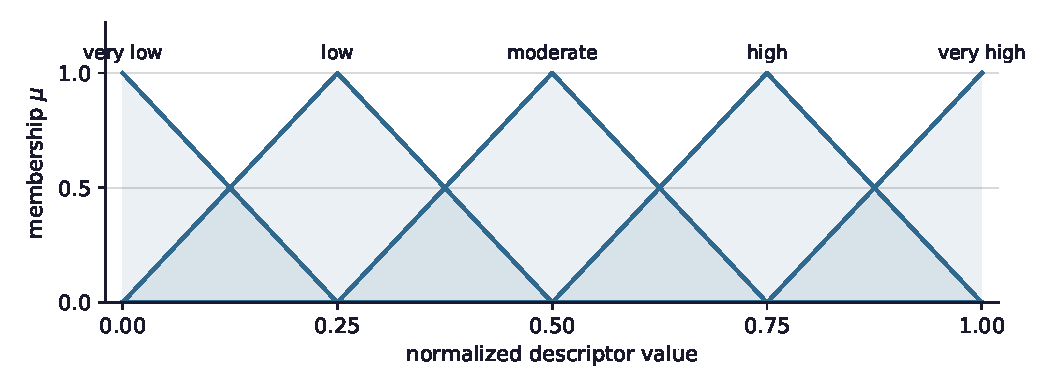
\includegraphics[width=0.85\textwidth]{figures/membership_functions.pdf}
    \caption{The five triangular membership functions over the normalized descriptor range. Each normalized value belongs to at most two adjacent linguistic terms, with memberships summing to 1.}
    \label{fig:membership}
\end{figure} Because several V3 descriptors are heavy-tailed (e.g.\ total note count, window maxima), a plain min-max normalization would compress most pieces into the lowest term. Instead, each descriptor is normalized by its empirical cumulative distribution function (CDF) on the training fold: a value is mapped to the fraction of training pieces at or below it, so that ``moderate'' corresponds to the corpus median regardless of the descriptor's raw scale. Values in the validation and test folds are clipped to $[0, 1]$ before fuzzification. A plain min-max variant is evaluated as an ablation in Section~\ref{sec:auxiliary}.

\subsection{Complete Search of Primitive Rules}
A primitive rule has the form ``if descriptor $X$ is term $T$ then class $C$.'' For every descriptor--term pair and class, the relevance of the corresponding rule is estimated on the training fold as
\begin{equation}
    R(C, X, T) = P(X \text{ is } T \mid C) \cdot \bigl(1 - P(X \text{ is } T)\bigr),
    \label{eq:fuzzy_relevance}
\end{equation}
where the fuzzy probabilities are estimated as mean memberships over the corresponding pieces~\cite{vatolkin2015interpretable}. The first factor rewards terms that are typical of class $C$; the second penalizes terms that are typical of the corpus as a whole, so that a term satisfied by almost every piece (uninformative) scores low even if it happens to hold for most of class $C$. For each class, the 32 descriptors $\times$ 5 terms are ranked by relevance, and a prediction is made by averaging the truth of the top-$m$ rules per class and taking the argmax over classes. The number of rules $m$ is selected per fold on the validation split by balanced accuracy, then the rule ranking is refit on the combined training and validation data before scoring the test fold.

\subsection{Fuzzy Pattern Trees}
A fuzzy pattern tree (FPT) represents one class as a single tree whose leaves are fuzzy statements and whose inner nodes are fuzzy operators --- here, \emph{and} (minimum), \emph{or} (maximum), and \emph{avg} (mean of the two children), following~\cite{senge2011topdown}. Leaves may additionally be negated (degree of truth $1 - \mu$), doubling the candidate statement pool to 320.

Induction is deterministic and top-down, one tree per class. The tree is initialized as the single statement minimizing the root-mean-squared error (RMSE) against the one-vs-all binary target on the training fold. At each step, every current leaf is considered for replacement by a new operator node whose two children are the old leaf and a new candidate statement; every (leaf, operator, statement) combination that does not push the tree beyond the maximum depth $d_{\max}$ is evaluated, and the extension with the lowest resulting RMSE is applied. Induction stops when no legal extension remains, the depth limit is reached on every branch, or the best available extension would worsen the error by more than a factor $(1 + \gamma)$, with $\gamma = 0.05$. $d_{\max}$ is swept over $\{1, \dots, 5\}$ and selected per fold on the validation split by balanced accuracy, mirroring the complete search's selection of $m$; $d_{\max} = 1$ yields a primitive, single-statement tree.

Because each one-vs-all target is a minority class (5--19\% positive across the eight classes), unweighted RMSE is minimized by trees that predict close to zero everywhere. Induction therefore uses a class-balanced RMSE by default, weighting positive and negative instances so that each contributes equally regardless of class size; a constant predictor then achieves its best possible (weighted) error at an output of 0.5, rather than at the majority class. The unweighted variant is evaluated as an ablation in Section~\ref{sec:auxiliary}, alongside a variant without negated leaves.
